\documentclass{article}
\usepackage{tikz}
\usetikzlibrary{arrows.meta, positioning, shapes.geometric}

\begin{document}

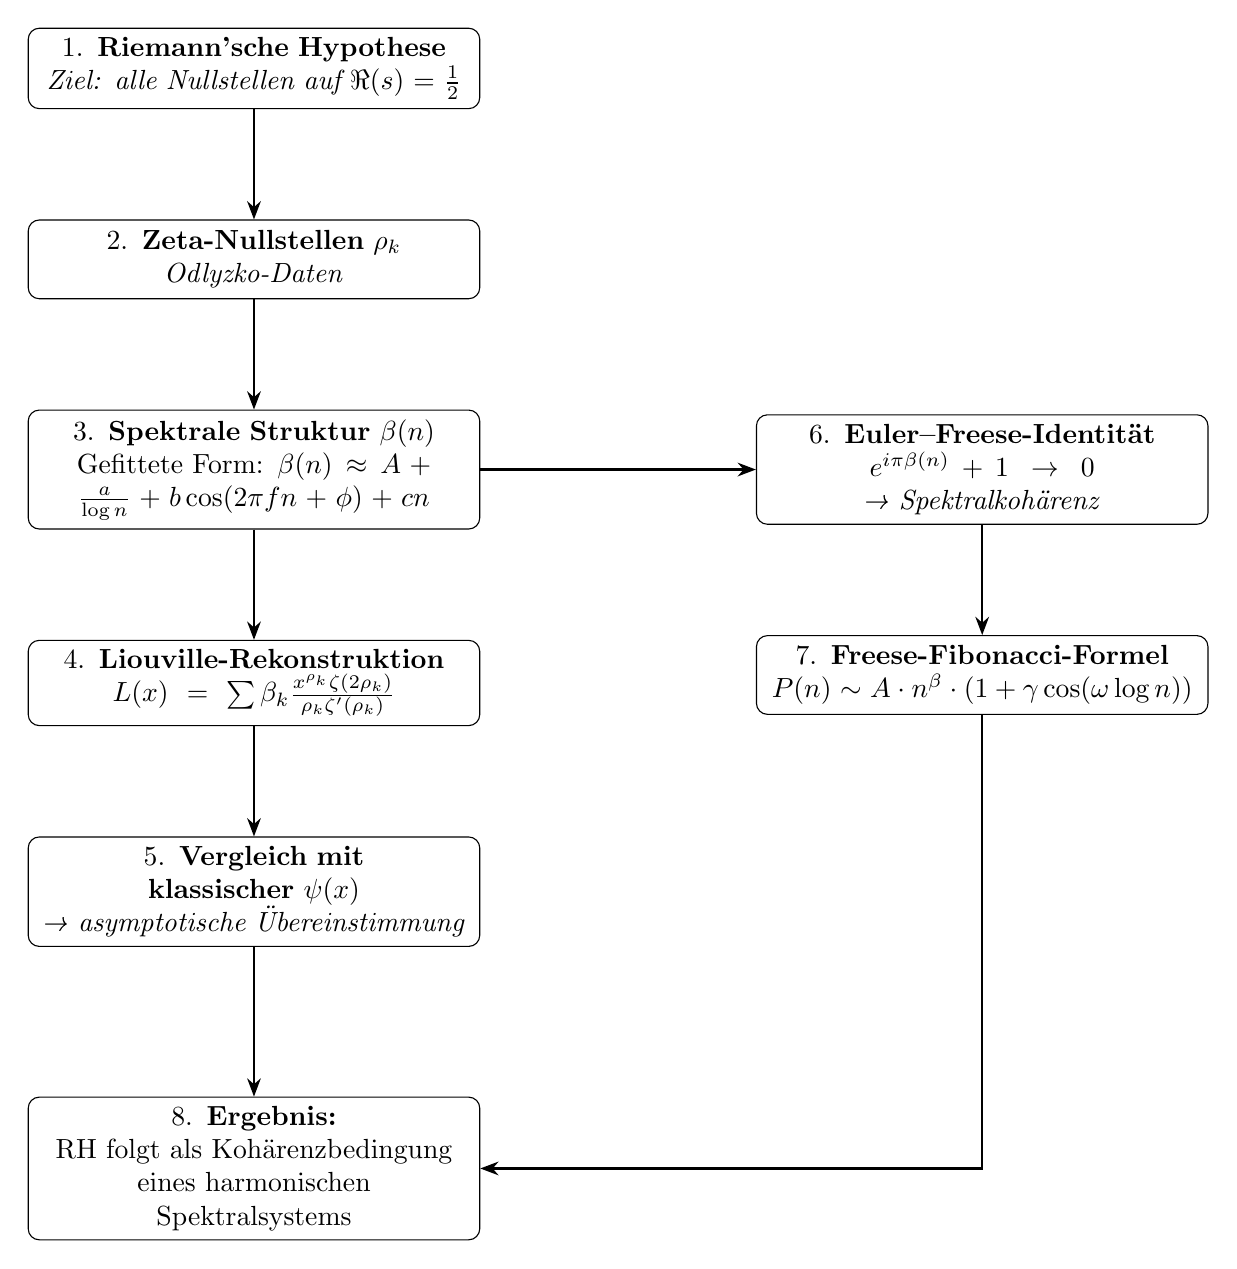
\begin{tikzpicture}[
  node distance=1.4cm and 3.5cm,
  box/.style={rectangle, draw, rounded corners, text width=5.5cm, align=center, minimum height=1cm},
  arrow/.style={-{Stealth}, thick},
]

\node[box] (rh) {1. \textbf{Riemann’sche Hypothese} \\ \emph{Ziel: alle Nullstellen auf $\Re(s) = \frac{1}{2}$}};
\node[box, below=of rh] (zeta) {2. \textbf{Zeta-Nullstellen} $\rho_k$ \\ \emph{Odlyzko-Daten}};
\node[box, below=of zeta] (beta) {3. \textbf{Spektrale Struktur} $\beta(n)$ \\ 
Gefittete Form: $\beta(n) \approx A + \frac{a}{\log n} + b\cos(2\pi fn + \phi) + cn$};
\node[box, below=of beta] (liouville) {4. \textbf{Liouville-Rekonstruktion} \\ 
$L(x) = \sum \beta_k \frac{x^{\rho_k} \zeta(2\rho_k)}{\rho_k \zeta'(\rho_k)}$};
\node[box, below=of liouville] (vergleich) {5. \textbf{Vergleich mit klassischer} $\psi(x)$ \\
\emph{→ asymptotische Übereinstimmung}};
\node[box, right=of beta] (eulerfreese) {6. \textbf{Euler--Freese-Identität} \\
$e^{i\pi\beta(n)} + 1 \to 0$ \\
\emph{→ Spektralkohärenz}};
\node[box, below=of eulerfreese] (fib) {7. \textbf{Freese-Fibonacci-Formel} \\
$P(n) \sim A \cdot n^\beta \cdot (1 + \gamma \cos(\omega \log n))$};

\node[box, below=of vergleich, yshift=-0.5cm] (fazit) {8. \textbf{Ergebnis:} \\
RH folgt als Kohärenzbedingung eines harmonischen Spektralsystems};

% Connections
\draw[arrow] (rh) -- (zeta);
\draw[arrow] (zeta) -- (beta);
\draw[arrow] (beta) -- (liouville);
\draw[arrow] (liouville) -- (vergleich);
\draw[arrow] (vergleich) -- (fazit);

\draw[arrow] (beta.east) -- (eulerfreese.west);
\draw[arrow] (eulerfreese) -- (fib);
\draw[arrow] (fib.south) |- (fazit.east);

\end{tikzpicture}

\end{document}